\documentclass[11pt, oneside, a4paper]{report}   %11pt font, one sided, A4, UK English
\usepackage [autostyle]{csquotes} %Fixes Quotation marks
\MakeOuterQuote{"} %Required for csquotes
\usepackage[utf8]{inputenc} %UTF-8 Encoding
\usepackage[colorlinks=true,urlcolor=magenta, linkcolor=red]{hyperref} %Colours links instead of highlighting with a box, URL's are Magenta
\usepackage{minitoc-hyper} %Used to give contents pages for individual chapters. Mini Tables of Contents.
\usepackage{graphicx}
\usepackage[final]{pdfpages}
\usepackage{tabulary}
\begin{document}

\begin{titlepage}
	\thispagestyle{empty}
	{\centering
		
\includegraphics[width=0.5\textwidth]{heriot-watt-logo.png}\par\vspace{1cm}
	%	{\scshape\LARGE Heriot-Watt University \par}
		\vspace{1cm}
		{\LARGE F29SO - Software Engineering\par}
		{\LARGE Stage 3 - Final Product\par}
		\vspace{1.5cm}
	%	{\scshape\Large Coursework\par}
		\vspace{1.5cm}
		{\scshape\LARGE\bfseries Final Report for Restaurant Ordering System by Buzzword \par}

		\vspace{3.5cm}
			\begin{center}
					April 5\textsuperscript{th} 2018
			\end{center}
		\vspace{1cm}
		\textit{Buzzword (Group 5)}\par
		\begin{tabulary}{\textwidth}{rcl|rcl}
			\\ \textsc{Kerr Brydon} & - & H00219387&
			\textsc{Wai Chong} & - & H00187212\\
			\textsc{Craig Duffy} & - & H00235298 &
			\textsc{Tommy Lamb} & - & H00217505 \\
			\textsc{Alastair Nibloe} & - & H00184083&
			\textsc{Mamta Sofat} & - & H00236213\\
			\textsc{Michael Steventon} & - & H00191545&
			\textsc{Michael Lones} & - & \textsc{Manager} \\
		\end{tabulary} \\
	
	}
\end{titlepage}

\dominitoc %Initialises the Domain of the MiniTOC
\tableofcontents
\pagebreak
\chapter{Marketing Analysis and Strategy}
\pagebreak
\pagebreak
\minitoc
\pagebreak
\section{Introduction}
\subsection{Executive Summary}
\begin{flushleft}
	The value of an effective marketing campaign can always go underestimated, through an effective marketing campaign it can increase awareness of a product and/or brand. In creating a dedicated marketing strategy it can allow businesses to target their intended customers and grab their attention. As a result of this it allows the company to grow their brand by selling their product or service.
	
	In this marketing plan the strengths and weaknesses of the product will be discussed also any opportunities and threats to the product. The surrounding environment of the product will also be evaluated through the use of a PEEST analysis, throughout this plan the target market, and also all the stakeholders who could potentially be affected by the system will also be discussed. Two of the final points to be discussed will be the marketing mix and then the unique selling point of the product.
	
	\subsection{Background}
	Buzzword Software has been given the task of creating a web application that allows waiters take customers’ orders and send them directly to the kitchen staff who can begin preparing the order as soon as the order is received. The client also requires that customers be able to view the status of their order and be given real time updates. To do this Buzzword Software created the Restaurant Ordering Support System (ROSS) which enables the staff and customers to do exactly what the client has requested.


\newpage
\section{Market Analysis}
When looking to enter into a new market with a completely new product it is important to review and analyse the surrounding market environment. To do this we studied similar products to ROSS which could be viewed as competitors and reviewed how they operate. It is important to also note how differently ROSS operates to our competitors. 

\subsection{Location}
As Buzzword software was founded and based in Edinburgh, it was agreed that this was the best place to enter the market. Due to the company’s proximity to the city as we are based at Heriot-Watt University, who have been kind enough to let us use their high-quality facilities to be able to carry out this project of building ROSS. Each team member also lives in Edinburgh or within commuting distance of the city, so this was agreed to be the best place to enter the market. 

Edinburgh as a city had an estimated 500,00 people living there in 2016 (Edinburgh Council, 2016) throughout the city there will be restaurants to cater for all tastes and cuisines and it is important for us to target the right ones. Edinburgh has more restaurants per head of the population than any other city in the UK, excluding London (Edinburgh Council, 2017). This backs up our decision to try and penetrate the market in Edinburgh. 

\subsection{Competitors}
After reviewing the competitors, it revealed that there is a lot of similar applications on the market, a lot of these are more targeted towards takeaways. These applications offer the ability to pay directly through the application. Any feature that many of the competing applications offer is the ability for the customer to order directly through the app. Thus removing any human interaction from the transaction.


\newpage

\section{SWOT Analysis}
\subsection{SWOT Diagram}
	\begin{figure}[!h]
	\centering
	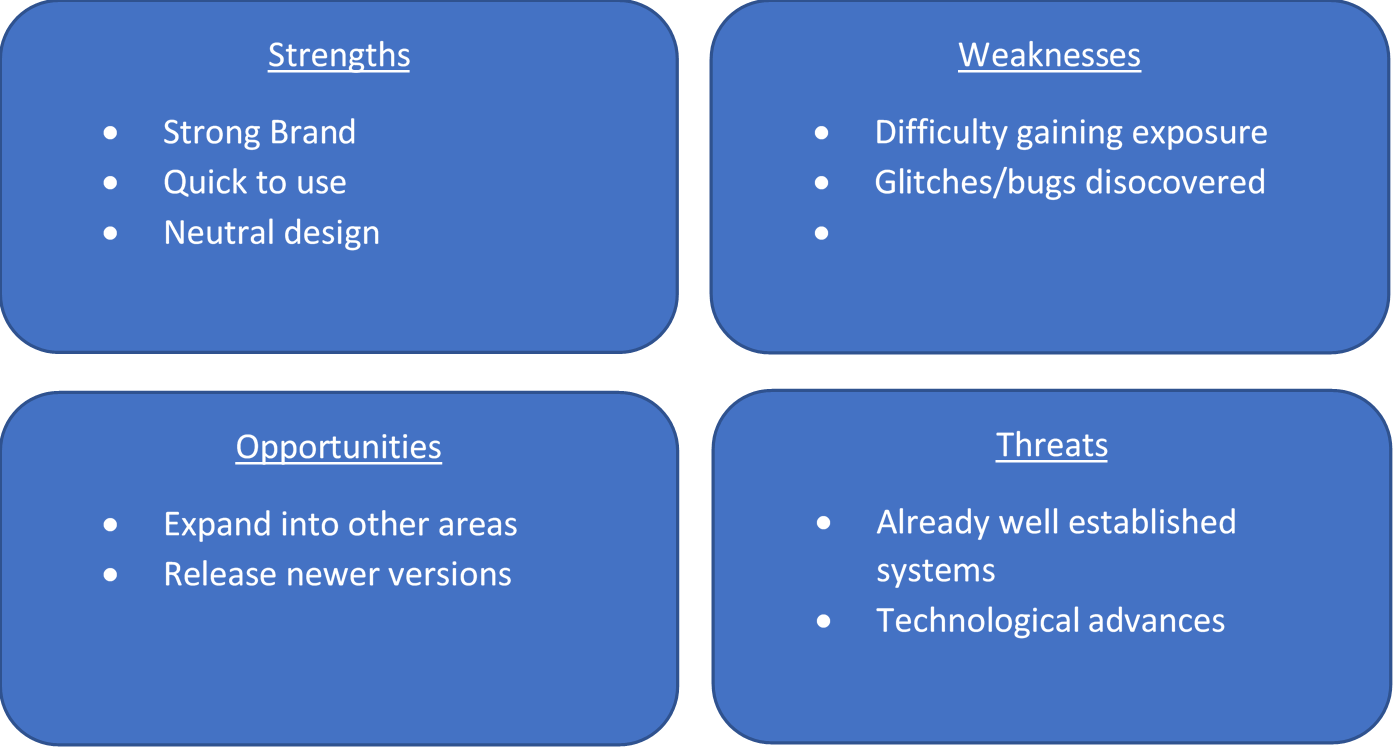
\includegraphics[width=0.7\linewidth]{SWOT_Diagram}
	\caption{SWOT Diagram for ROSS}
	\label{fig:swotdiagram}
	\end{figure}

\subsection{In depth SWOT Analysis}
\subsubsection{Strengths}
Our product, The Restaurant Ordering Support System (ROSS) has enabled us to create a solid foundation, which over time will hopefully develop over time into a strong brand. This will allow customers to instantly identify our products and they will associate our products with quality. 

Having no sign up to use the product means that customers of the restaurant will be able to use ROSS as soon as the order has been placed and no time at all will be wasted with signing up and creating passwords. This is a huge strength of ROSS as it also means that the customers of the restaurants will not be at risk of spam email after email. 

When designing the product, we thought it was best to use a neutral colour scheme as when in use at a restaurant it will be used by people of all different ages and different genders. This is thought to be the best option due to their be no single market segment to direct our design towards. 

\subsubsection{Weaknesses}
As Buzzword Software is a relatively new organisation in the software industry, it could be difficult to get our name out there. This could hinder the growth of our company and the software that we produce. Exposure is difficult to get as it takes time for a company to become known and be trusted by companies. 

Over time, as with any piece of software, the regular users of the software will discover various problems with the product. These would most take shape in the form of bugs and glitches, in order for our product to stand the test of time, regular maintenance would be essential. 

\subsubsection{Opportunities}
At this moment in time ROSS is only being developed for use in restaurant. However, in the future the system could be adopted for use in other industries, this is an opportunity that could be explored in future. One opportunity to look at could be a car garage providing updates to the owner of the car on how the repairs are going and an estimation of how long the repair will take. 

Another opportunity available to Buzzword software depending on the success of the system, would be releasing newer versions which added functionality. This added functionality could include customers being able to order and pay directly from their phone to make the customer’s experience even more enjoyable.

\subsubsection{Threats}
One of the main threats to our product ROSS is that well established systems may be more trusted by potential customers. Although these systems may have different ways of operating, they are still targeting the same target market as ourselves. 

Advances in technology mean that ROSS could be left behind by competitors’ systems, constant updates and work from the development team will ensure that ROSS doesn’t fall back and become outdated.

\newpage
\section{PEEST Analysis}
PEEST analysis is a marketing tool used by companies to analyse the surrounding environment that they are operating in. This analysis will allow us to examine the political and legal, economic, social, technological and environmental issues which could affect the organisation or the system or the way in which the system works. Before an organisation releases a new product, it is best to analyse the external environment and evaluate how this could affect the release of the product.
\subsection{Political and Legal}
The United Kingdom is currently going through an unprecedented time of uncertainty due to the “Leave” vote in the referendum on whether Britain should leave the European Union. This could have an impact on how willing companies are to invest in technology such as ours. It is important that all laws be abided by the company, such as no breaches of the Data protection act of 1998, and all working time regulations are adhered to.
\subsection{Economic}
There are many economic factors for our company to consider that could have an adverse effect on ROSS. If a recession was to occur, similar to 2008, companies will begin to look where they can save money and may see ROSS as a product to invest in when the times aren’t as tough for consumers. 
\subsection{Environmental}
As ROSS is a software program which utilises different pieces of hardware, environmental concerns are one of the biggest issues the company will face. However it is important to ensure that Buzzword Software strives to recycle all paper and plastic where possible and ensure to save electricity by ensuring all computers are switched off when not in use. 
\subsection{Social}
Nowadays peoples’ lives are busier than ever and technology is relied upon more than ever. By using technology to speed up the process between ordering food and it actually being ready to be consumed by the customers it can create extra time for people. Nowadays more and more people are going out and visiting restaurants, according to PWC(2017) the number people eating out at restaurants has increased year on year since 1989. 
\subsection{Technological}
Technology is ever changing and improving rapidly, it is important that the system is accessible for different mobile operating systems (iOS, Android etc) and is portable between browsers (Google Chrome, Safari etc). 

\newpage
\section{Target Market}
The target market of an organisation can be defined as the group of consumers or businesses that the product is being targeted towards. 

In order to choose our target market, we had to carry out a task called Market segmentation, this is where individuals or organisations are grouped together based on similar characteristics, which allows the company to then pick the most attractive segment to target. For example, fast food chains such as Burger King and McDonalds were grouped together as they have similar characteristics. By doing this it allows the selling company to be able to create an undifferentiated marketing strategy for the whole segment. 

After much consideration and research into the topic, it was decided that the market we shall aim our product towards would be medium to large restaurant chains, i.e. Nando’s or Frankie and Benny’s. Nando’s currently has over 300 UK restaurants (Gander, 2017) and Frankie and Benny’s operates over 200 sites in the UK (Marston, 2016). The reasons behind this decision were that these chains would have the money available to invest in such a system and if we secured the business of a restaurant chain it would mean Buzzword software would in turn make more money, due to the increased locations the system would be needed. 

Smaller independent restaurants were considered but after initial research we discovered that the management running the restaurant may not have the resources to accommodate the system. Fast food chains (i.e. McDonalds and Burger King) were also considered but because the food is ready quickly is seemed pointless having a system that tracks the customers wait time, when the customer expects the food instantly. However this does not mean that smaller independent restaurants and fast food chains can’t purchase and use ROSS, this just means we as a company are not targeting our system towards them. 

\newpage
\section{Stakeholders}
When a company purchases ROSS many different stakeholders will be affected by the purchase and also the implementation of the system. Chris Fill (2006) recommends that stakeholders of an organisation be organised into four main groups. These four groups are: Employees, Customers, Financial Group and Organisations and Communities, to ensure the success of the system all four of these groups needs must be met to ensure the longevity of the system. In this system we will look to identify the different stakeholders who are involved with ROSS. 
\subsection{Waiting Staff}
Category: Employees
\linebreak
Waiting staff will be one of the primary users of the system as they will be taking the customers orders, which will then be sent to the kitchen staff. It is important for us to hear directly from the waiting staff as we will be able elicit requirements and be notified of any problems or glitches with the system. The waiting staff will be doing the majority of their work with the system, so it is imperative it works as specified. 

\subsection{Kitchen Staff}
Category: Employees 
\linebreak
Kitchen staff will also be one of the main users of the system as they will be receiving the orders from the waiting staff via ROSS. Similar to the waiting staff it is important for feedback from the kitchen staff to be fed back to the development and maintenance, so any bugs or glitches can be fixed. 

\subsection{Restaurant Patrons}
Category: Customer
\linebreak
One of the most important stakeholders are the customers who will be using the restaurant. They will be directly benefited by the implementation of ROSS. The customers of the restaurant have to be considered as an important stakeholder as they are one of the primary users of the system and their views on the system are important. 

\subsection{Heriot-Watt University}
Category: Financial Group 
\linebreak
The financial group behind this ambitious project is Heriot-Watt University, they have provided Buzzword Software with the tools and resources to be able to carry out the design and implementation of the system. Heriot-Watt were the driving force behind the project and assigned Buzzword Software to this

\subsection{Unite Trade Union}
Category: Organisations and Communities
\linebreak
Consulting with the trade union for restaurant and kitchen workers would be beneficial as some workers may be worried that ROSS may be replacing them. To alleviate these fears interacting with the trade union and creating a dialogue would go a long way to ensuring the system is implemented without any major problems or protests from staff.


\newpage
\section{The Marketing Mix}
The marketing mix, or 4 P’s as some call it, was introduced by E. Jerome Mccarthy in 1960. These 4 elements focus on getting the right product in the right place at the right price, no one element is more important than the other and each element is there to support the others. 
\subsection{Product}
ROSS does exactly what the customer needs and requires it to do. Our product will not be for sale to the public due to the nature of ROSS, all the transactions involving our product will be directly to other businesses (B2B). The product will enable waiters to quickly send orders to the kitchen staff who will receive the orders quicker and can begin preparations to the customers meal straight away. One of the features which makes ROSS stand out from the crowd is that it doesn’t require the user to sign up, by designing the system in such a way, it allows the customer to instantly check the status of their order instantly. 
\subsection{Place}
There is two aspects to the place element of the marketing mix in the case of ROSS, the first element of this where the actual system is based. ROSS is based online due to the way the system operates through the need to be able send orders and for the customers to be able to check the status of their order. Customers would access this application through a website on the internet, due to the high number of people who now own smartphones with internet capabilities it was decided that this was the best method accessing the system. 
\subsection{Price}
To promote our product to potential customers, we have to select the strategy for doing so and the mediums used to do so very carefully. One of the most effective methods would be to contact the companies that we are targeting directly and show how much more efficient their restaurants could be run purely by using our system. One way in which this could be done, is by inviting the management of the restaurants to an open demonstration of our system so they could see for themselves just how the system would actually work in practice and not just in theory. 
\subsection{Promotion}
The pricing strategy for ROSS is crucial to how well the system will fare in todays market. We needed to select a price which wasn’t too expensive as this would drive potential customers away and come to a price that wasn’t too cheap as Buzzword would lose money. In order to be able to compete with well established restaurant ordering systems, it was agreed that a competitive pricing strategy shall be adopted for the product where we shall adopt the same pricing structure as our competitors to allow us to compete with them. 


\newpage
\section{Revenue Model}
A revenue model is a framework for investigating how a product or service will actually make money. 

The main way for ROSS to generate money for Buzzword Software would be a restaurant paying for the system, and Buzzword installing the software and hardware in the premises. This is the easiest and most common way of making money.

Another way for ROSS to make money is for a lite version of the software to be released. The waiting and kitchen staff applications would be unaffected in this version; however the customer application would have advertisements at pre-agreed areas, and in return the restaurant purchasing the software would be able to purchase ROSS for a discounted price. This is a common method in the development world, and if the restaurant wanted to upgrade the full version with no advertisement this could be accommodated.

\newpage
\section{References}
\begin{itemize}
	\item Edinburgh.gov.uk. (2016). Edinburgh's population | Population of Edinburgh | The City of Edinburgh Council. [online] 
	Available at: 
	\linebreak 
	http://www.edinburgh.gov.uk/info/20247/edinburgh\_by\_numbers/34/population\_of\_edinburgh/1
	[Accessed 27 Mar. 2018].
	\item Fill, C. (2006). Simply marketing communications. London: Pearson.
	\item  Gander, K. (2017). It turns out you were learning to love peri-peri long before we ever had Nando's. [online] The Independent. 
	\linebreak
	Available at: https://www.independent.co.uk/life-style/food-and-drink/nandos-peri-peri-chicken-origin-rise-popularity-spice-levels-uk-restaurant-a7846706.html 
	
	[Accessed 26 Mar. 2018].
	\item Marston, R. (2016). Frankie \& Benny's owner to close sites. [online] BBC News. 
	\linebreak
	Available at: http://www.bbc.co.uk/news/business-37193629 
	
	[Accessed 27 Mar. 2018].
	\item PwC. (2017). Restaurants 2017: Food for Thought. [online] 
	\linebreak
	Available at: https://www.pwc.co.uk/services/business-recovery/insights/restructuring-trends/restaurants-2017-food-for-thought.html 
	
	[Accessed 27 Mar. 2018].
\end{itemize}
\end{flushleft}
%%%%%%%%%%%%%%%%%%%%%%%%%%%%%%%%%%%%
%%%%%%%%%%%%%%%%%%%%%%%%%%%%%%%%%%%%
%%       END MARKETING        %%%%%%
%%%%%%%%%%%%%%%%%%%%%%%%%%%%%%%%%%%%
%%%%%%%%%%%%%%%%%%%%%%%%%%%%%%%%%%%%
\chapter{Final Usability Evaluation}
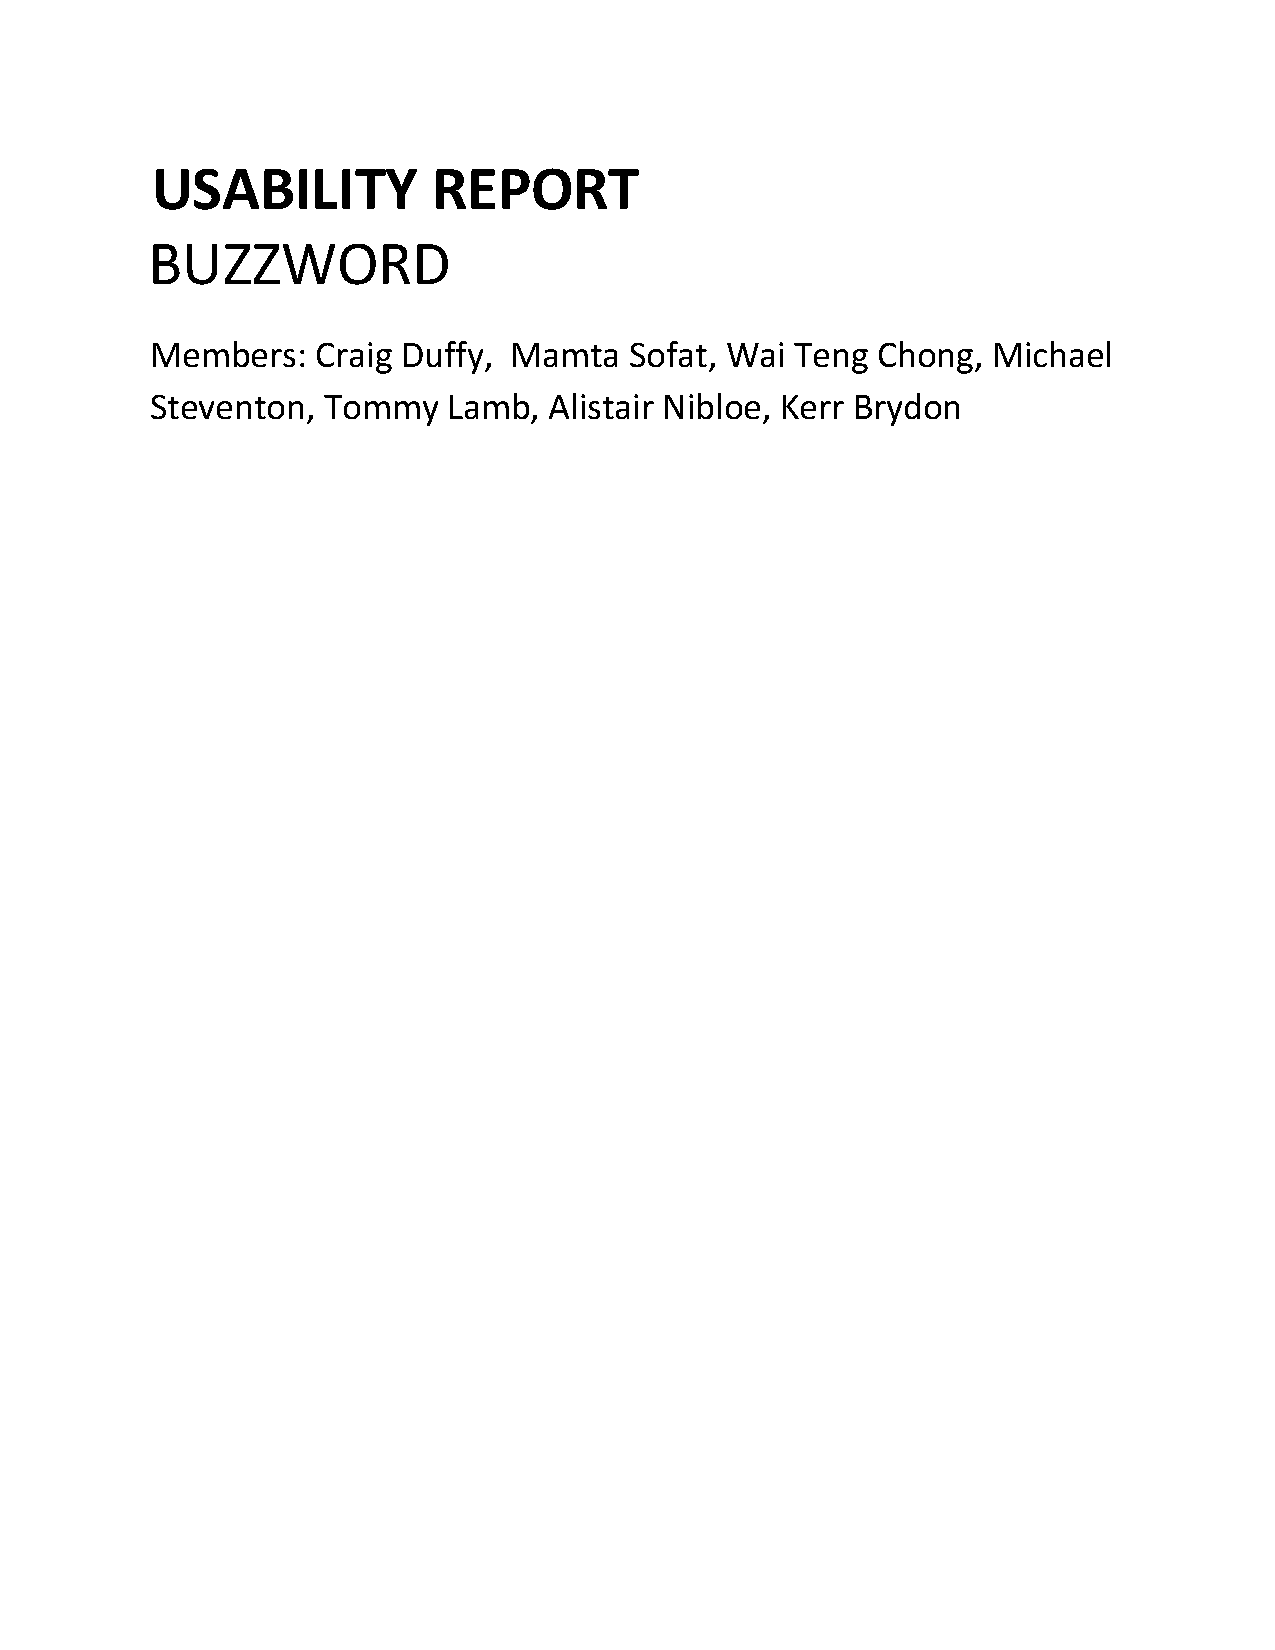
\includepdf[pages= 1-21]{usability.pdf}

%%%%%%%%%%%%%%%%%%%%%%%%%%%%%%%%%%%%
%%%%%%%%%%%%%%%%%%%%%%%%%%%%%%%%%%%%
%%       END USABILITY        %%%%%%
%%%%%%%%%%%%%%%%%%%%%%%%%%%%%%%%%%%%
%%%%%%%%%%%%%%%%%%%%%%%%%%%%%%%%%%%%
\chapter{Final Application Design and Implementation}
\pagebreak
\minitoc
\pagebreak
\section{System Overview}

The technologies used in the system, for the most part, are the same as were planned in stage 1 of this project. The system was developed and deployed on the Linux-based server available to students within the MACS department, using MySQL as the supporting database and Apache HTTP server to serve static HTML and execute server-side PHP scripts -- both also available within the department. The only change from the original plan was the choice to not use the React framework. We decided to forego any frameworks as the scope and scale of the project was limited enough that scalability posed no issue -- a major advantage of React -- and the ramp-up time for the team would have been prohibitively expensive. Any other advantages were relatively minor, and insufficient to offset the cost in learning the technology. As such all functionality was implemented using purely standard JavaScript, alongside HTML and CSS, with PHP and SQL as server-side technologies.

Architecturally the system is deficient and in violation of the original plan to a significant degree, as the result of design decisions made by individual implementers too close to the project's delivery date. The original plan which was maintained for most of the project's duration called for three client-side-only applications, namely the Waiting, Kitchen, and Customer components, which would interact exclusively through a set of server-side scripts, collectively the Server component. This Server component was to be solely responsible for interacting with the database, and all communication was to be carried out using asynchronous JavaScript-based requests and JavaScript Object Notation (JSON) structured data, which is specified in the Component Communication Specification appendix. The complete database and most Server functionality was implemented according to this plan, which the Waiting component also follows. Alas those components are alone in that. The Kitchen and Customer components both use bespoke PHP server-side scripts which directly access the database, with no use of the Component Intercommunication Specification since they completely ignore the implemented Server component and its API. The problem with this is it tightly couples the User Interface to the data representation in the database. According to the plan, a database change would only affect the Server component; with the API and JSON data unchanged, each client-side application would be none the wiser. As implemented however, most of the Kitchen and Customer components would need to be re-engineered to account for the change. On top of that there is the wasted man-hours spent drawing up the JSON and API specification and implementing the unused scripts for the Server component, as well as lowered system-wide component cohesion and future scalability.

The consequence of this is exceptionally convoluted dataflow for a system of this limited size, with the lines between components blurred somewhat as there are effectively two different architectures in use. 

\section{"Describe your implementation methodology. Did you use iterations, SCRUM or other agile
techniques?"}
We initially set upon SCRUM as our implementation methodology, with sprints based on the plan submitted in the Stage One document. This, however, was quickly abandoned and a more "ad lib" approach was taken to implementation. This is discussed in detail in the Project Evaluation as being a bad idea.

\section{"Summarise how you tested the final system for technical correctness."}

The system was "tested" for technical correctness by performing mock orders during our run-throughs and making sure the results were as expected. This is not a good example of testing, and is by no means exhaustive. A proper testing framework should have been used.
\section{Installation and Maintenance}

The first stage in installing the system is to setup a network connected computer with the appropriate third-party software. The system was implemented and tested on the open-source Linux operating system, however other operating systems may work. Likewise other PHP-server software and any other standard-compliant SQL database may be sufficient, however the open-source Apache server and MySQL database software is recommended as these are the targeted technologies. Installation and maintenance instructions for this software should be sought from their respective vendors. An appropriate Local Area Network is also required in the premises, the specific implementation of which is largely unimportant. Note that our software implements no access-control for specific web-pages, such as the Kitchen component, and this should be implemented at the network level and/or in server software. It is suggested that declaring static IP addresses or sub-netting for staff devices be used, as server software can restrict access based on a client's IP address.

Once that is complete, the database should be instantiated. SQL scripts are included to create the necessary tables and populate them with data, designed for MySQL. The data that is loaded into the database is read from individual text files, named "<DBTableName>Data.txt", as a sequence of tab-separated values with Linux newline characters (\textbackslash n) separating database records. Using a heading line each file specifies explicitly for which fields of the table, and in what order, data should be entered. The structure of JSON data held within the database, such as for menus, is as defined in the Component Communication Specification appendix. Please note that our software assumes a UTF-8 character encoding, which may not be the default for the database software. Other character encodings may cause data corruption, particularly if using characters featuring accents.

The HTML, JavaScript, CSS, and PHP files should be deployed according to the instructions for the server software being used, with some modification. All PHP files need to be updated with the URL and login details of the database deployed previously. Equally any absolute URLs used in \textbf{any} file will need to be updated, as may some relative URLs, depending on the file structure where the files are deployed.

No provision is made in the system as currently implemented to allow end-user maintenance of the system. Third-party software and hardware notwithstanding, the system is however relatively low maintenance. Currently the only maintenance recommended is to delete completed orders from the database at close of business each day. The exact interval for this preventative maintenance is dictated by server hardware, and therefore may be extended significantly on systems with higher storage and/or computational performance but is neither recommended or guaranteed. 
%%%%%%%%%%%%%%%%%%%%%%%%%%%%%%%%%%%%
%%%%%%%%%%%%%%%%%%%%%%%%%%%%%%%%%%%%
%%   END APPLICATION DESIGN   %%%%%%
%%%%%%%%%%%%%%%%%%%%%%%%%%%%%%%%%%%%
%%%%%%%%%%%%%%%%%%%%%%%%%%%%%%%%%%%%

\chapter{Project Evaluation} 
\pagebreak
\minitoc
\pagebreak
\section{Organisation} \label{sec:Organisation}
\subsection{"How was your group organised? Was it successful?"} \label{sec:Organisation - 1}

The organisation of Buzzword varied dramatically during the three distinct stages of the project:  \\ \\
At Stage One the group worked in small teams of two or three to complete a delegated section of the 
specification document each: this was determined by the Organisational Manager and was 
determined to be the best course of action for the project at this particular time as, since each section awarded 
relative autonomy (e.g. The Requirements Analysis does not depend on the Risk Analysis and vice versa), groups 
could organise themselves easier with less people which, in theory, would have reduced the overhead of working as a team. \\ \\
At Stage Two, the group was split into a "Core Dev" team and a "Web" team containing three people each and with the Organisational
Manager being involved in both teams. The idea here was that one team would focus all its efforts on the Company Website and subsequent 
branding etc. while the other team focused on developing the main application; the Organisational manager would help out where possible 
then handle the Progress Report section. Much like Stage One, the core motivation was to reduce the burden of "people management" and 
allow teams to organise themselves with a better focus on what is important to them with less conflict of schedules being awarded by having less
people.\\ \\
At Stage Three, the group took on a hybrid organisation of Stages One and Two: the "Core Dev" team remained as a small team but gained one
member from the "Web" team, while the "Web" team disbanded into two separate individuals who could on the tasks of the "Marketing Analysis and Strategy"
and, once the application was complete, the " Final Usability Evaluation" without relying on anyone else. Like the previous two organisational methods 
the strategy was very much to split the work into distinct sections people could work on without relying on others and this was true throughout the whole project.\\ 

It is the view of Buzzword that this approach was ill-thought-out and poorly adhered to. While the "divide and concur" nature of the approach could have the 
opportunity to be successful; more frequent, whole group and team, meetings would have greatly aided the project's progress. 
As everyone was, for the most part, able to work on a section independently there was miscommunication about the intended overview of the system and 
implementation strategy, and while we did mange to produce a functioning application the end product could have been greatly improved by more 
frequent reporting from each member to the rest of their team, the group as a whole, and to the Organisational Manager as well as the group manager.\\ 
In any theoretical future projects, we would aim to have daily standup "SCRUM" meetings for each of the teams, as well as a weekly meeting where each member
can report on their progress to the rest of the group, as well as the Organisational Manager, and the group manager.  
\subsection{"How well did your group collaborate? How did you handle any problems which arose?"} \label{sec:Organisation - 2}
We made a reasonable attempt to collaborate well, but due to the organisational strategy outlined above this was largely not required from the group. Very few sections, 
with the exception of cross communication of the components in the "Core Dev" team required members to be dependant on others/work on the same document 
together. That being said, there was a positive "team sprit" with reasonable turnout during group meetings and only one member absent without explanation during during
the Stage Two demonstration to the group manager. Thought the project, limited problems arose due to the organisational strategy however;  there were bereavements from 
certain members resulting in delays to their sections of work, as well as difficulties with group meetings during the period of industrial action experienced by Heriot-Watt University.
The former was handled by simply accepting and accounting for the delays that were inevitable, and the former was handled by working to the best of our ability independently and 
communicating via a group chat.
\subsection{"How successful were the timings in your original plan?"} \label{sec:Organisation - 3}
Not at all. From Week One of the original implementation plan the organisation and structure of the SCRUM methodology of which the plan was based around was immediately 
abandoned. The group intended to get "back on plan" but the disruption to ordinary working schedules awarded by examinations and the holiday period were not suitably accounted 
for in the plan. As such, by the time the holidays were over and normality had returned the group were so far off track that it was no longer practical to attempt to follow the plan 
which had been originally outlined. An "ad-lib" approach was taken to planning for the rest of the project prioritising must have functional requirements, and sections which were most
urgently due. 
\pagebreak
\section{Implementation}
\textit{It is assumed that "Implementation" here refers solely to the coding and development of the application and not the implementation of the project as a whole}
\subsection{"What was your implementation schedule and how did this differ from the original plan?"} \label{sec:Implementation - 1}
Our implementation schedule consisted of a short burst at the start of Stage Two where the server was implemented, followed by a hiatus until shortly before the Stage Two deadline, followed by a short burst where some 
functionality of each of the components was implemented, followed by another hiatus until shortly before the Stage Three deadline, followed by a short burst where the remaining application was developed. Exact timings 
and what was accomplished when can be obtained by viewing the commit history of the project's GitHub repository in the Appendix. This differed immensely from the original plan of frequent and gradual development of
each of the requirements as opposed to the bursts experienced. 
\subsection{"Was your implementation approach successful (e.g., SCRUM, other agile, etc.)? Why or why
not?"} \label{sec:Implementation - 2}
It could be argued that our implementation approach was not unsuccessful with a reasonable product being developed and delivered at the end of the project. However, this comes with the significant caveat that we did not 
achieve everything we had planned, and the end product was not of as high quality as we would have liked. The group feels the implementation approach, therefore, was unsuccessful but this was not a result of the planned 
implementation methodology adopted but rather that it was not adhered to at all.  
\subsection{"Which languages, tools, and techniques did you use? How suitable were they?"} \label{sec:Implementation - 3}
For this project we used HTML5 and CSS3 for the Front End along with a Linux, Apache, MySQL, PHP (LAMP) server for handling data moving between components. Some PHP and Javascript was used in the Front End but the majority of PHP is used in the backend. While this approach did not afford us some fancy features such as the ability to save the WebApp as an offline application on mobile devices it was more than appropriate for the task at hand and accomplished the functionality. It was determined that we should "stick to what we know" rather than spend time and resources learning a framework/other language which likely would not benefit us much in this situation.
\pagebreak
\section{Product} 
A most of the core functionality required by the specification document has been implemented. A notable omission is the inclusion of the ability for a waiter to amend an existing order; this has cascading consequences where a number of our "Could Have" or "Should Have" requirements were not implemented as these related to the amendment of orders. 
\subsection{"How many of your requirements did you meet?"}
The table below references our Stage One - The Bid document and outlines each of the Functional Requirements with indications of the degree to which each of these were implemented.\\
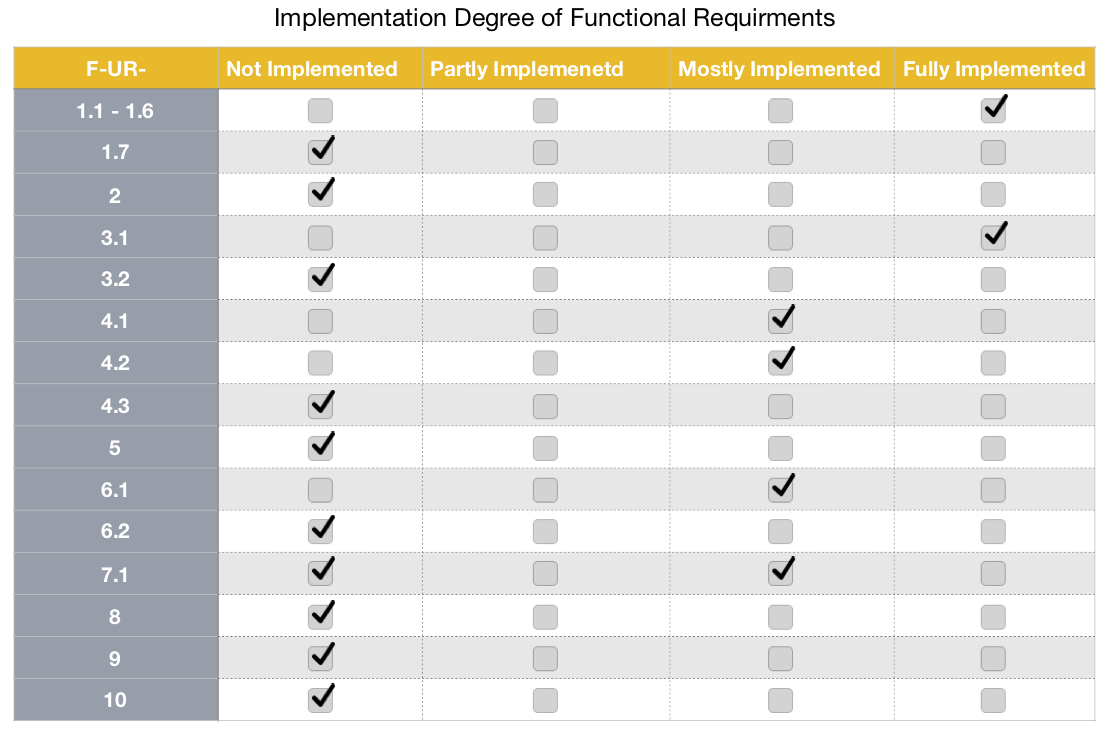
\includegraphics[width = \textwidth]{FR.png}
\subsection{"What is particularly special about your product? Have you included extra features?"}
The key selling point of our application is the ability to perform the requested functionality without the need for either the customer or the waiter to have/create an account. We felt that account creation would be cumbersome for the user and as such deliberately avoided it. No extra features have been included outside of what was outlined in our original requirements document. 
\subsection{"How robust is your final system? Are there known bugs or constraints?"}

The resulting system is fairly robust however there are a couple known bugs: \\
\begin{itemize}
  \item Kitchen does not display correct timers for orders with numbers shared by other orders in the system
  \item Customer does not display the ETA of an order
  \item Kitchen does not display some menu items (though are in DB and Customer component shows them)
  \item Server does not check the "correctness" of JSON it returns 
\end{itemize}
The known constraints are anything that has not been implemented from the Requirements Specification.

\subsection{"How usable did your subjects find the final system?"}
We ran a usability study on 6 participants to test the usability of our application. The consensus from these participants appeared to be that the application functioned well enough and the information hierarchy was reasonable but the usability of the application could be greatly improved by redesigning, and improving the aesthetics of the application: making things bigger/more readable and easier to follow. For more information on our findings please refer to the "Final Usability Evaluation" chapter of this document.
%%%%%%%%%%%%%%%%%%%%%%%%%%%%%%%%%%%%
%%%%%%%%%%%%%%%%%%%%%%%%%%%%%%%%%%%%
%%       END EVALUATION       %%%%%%
%%%%%%%%%%%%%%%%%%%%%%%%%%%%%%%%%%%%
%%%%%%%%%%%%%%%%%%%%%%%%%%%%%%%%%%%%
\chapter{Appendix}
\section{Website}
The Company Webpage is available at: \\
\url{http://buzzwordSoftware.uk/}
\section{GitHub}
The Project GitHub Repo is available at: \\
\url{https://github.com/CraigJDuffy/Buzzword}
\section{Hosted Application}
The Application is hosted at: \\ 
\url{www2.macs.hw.ac.uk/~til1/ThirdYear/GroupProject/}\\
Then the specific components are at: \
\begin{itemize}
\item Waiting/index.html
\item Kitchen/kitchen.php
\item Customer/html/checkOrder.html
\end{itemize}

\section{Component Specification Document}
The Component Specification Document is available on the next page: \\
\pagebreak
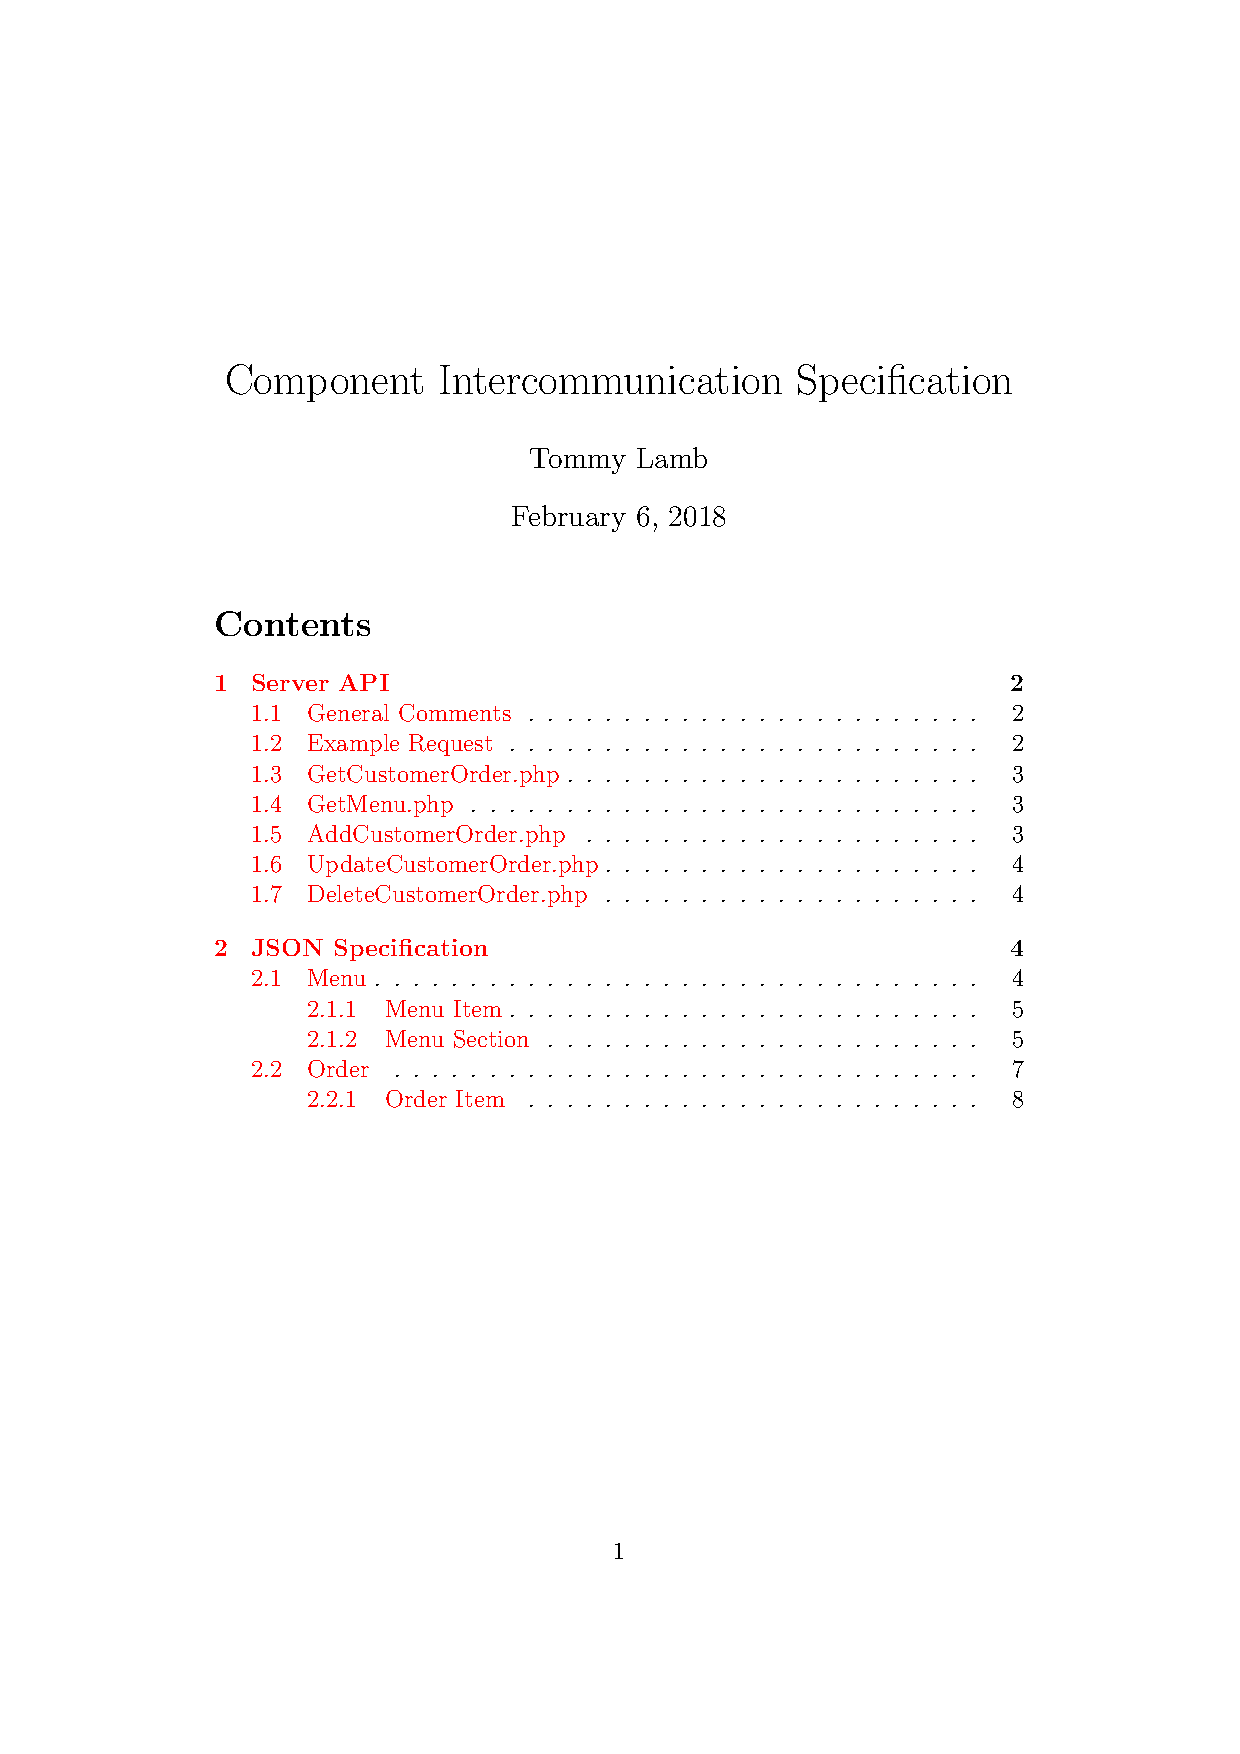
\includepdf[pages=-]{ComponentComunicationDocumentation.pdf}
\pagebreak


%%%%%%%%%%%%%%%%%%%%%%%%%%%%%%%%%%%%
%%%%%%%%%%%%%%%%%%%%%%%%%%%%%%%%%%%%
%%             END            %%%%%%
%%%%%%%%%%%%%%%%%%%%%%%%%%%%%%%%%%%%
%%%%%%%%%%%%%%%%%%%%%%%%%%%%%%%%%%%%
\end{document}